% LaTeX Template For MATH 490 @ VCU
\documentclass[12pt]{book}

\usepackage{hyperref}
\usepackage{amsmath}
\usepackage{amsthm}
\usepackage{amssymb}
\usepackage{enumerate}
\usepackage{enumitem}
\usepackage{titlesec}
\usepackage{multicol}
\usepackage{multirow}
\usepackage{mathtools}
\usepackage{mdframed}
\usepackage{tocloft}
\usepackage{tcolorbox}
\usepackage{extarrows}
\usepackage{libertine}
\usepackage[libertine]{newtxmath}

\setlist{nosep}
\setlist[enumerate]{label=\roman*.}

\renewcommand{\arraystretch}{0.85}

\definecolor{defcolor}{RGB}{255,236,236}    % light red
\definecolor{ngtcolor}{RGB}{255,242,242}    % lighter red
\definecolor{lnkcolor}{RGB}{0,0,180}        % blue
\definecolor{thmcolor}{RGB}{236,236,255}    % light blue
\definecolor{lemcolor}{RGB}{239,239,255}    % lighter blue
\definecolor{procolor}{RGB}{242,242,255}    % lighter lighter blue
\definecolor{crlcolor}{RGB}{245,245,255}    % lighter lighter lighter blue
\definecolor{xmpcolor}{RGB}{255,240,225}    % light orange
\definecolor{rmkcolor}{RGB}{233,255,235}    % light green
\definecolor{axicolor}{RGB}{255,255,233}    % light yellow
\definecolor{notcolor}{RGB}{255,255,244}    % lighter yellow
\definecolor{whacolor}{RGB}{250,250,250}    % lighter gray
\definecolor{reccolor}{RGB}{255,244,255}    % lighter purple

\hypersetup{
    colorlinks,
    citecolor=lnkcolor,
    filecolor=lnkcolor,
    linkcolor=lnkcolor,
    urlcolor=lnkcolor
}

\newtheoremstyle{break}
    {\topsep/1.5} % space above
    {\topsep/2.2} % space below
    {}          % body font
    {}          % indent amount
    {\rmfamily} % theorem head font
    {.}          % punctuation after theorem head
    {0.5em}  % space after theorem head
    {\textbf{\thmname{#1}\thmnumber{ #2}}\thmnote{\text{ (#3)}}}
                % theorem hed spec. (empty = "normal")

\newtheoremstyle{no_label}
    {\topsep/1.5} % space above
    {\topsep/2.2} % space below
    {}          % body font
    {}          % indent amount
    {\rmfamily} % theorem head font
    {.}          % punctuation after theorem head
    {0.5em}  % space after theorem head
    {\textbf{\thmname{#1}\thmnumber{}}\thmnote{\text{ (#3)}}}
                % theorem hed spec. (empty = "normal")

\theoremstyle{break}
\newmdtheoremenv[
    backgroundcolor=thmcolor,
    linecolor=black,
    linewidth=1pt,
    topline=true,
    bottomline=true,
    rightline=true,
    skipabove=\topsep/1.5,
    skipbelow=\topsep/2.2
]{theorem}{Theorem}[section]
\newmdtheoremenv[
    backgroundcolor=crlcolor,
    linecolor=black,
    linewidth=1pt,
    topline=true,
    bottomline=true,
    rightline=true,
    skipabove=\topsep/1.5,
    skipbelow=\topsep/2.2
]{corollary}[theorem]{Corollary}
\newmdtheoremenv[
    backgroundcolor=lemcolor,
    linecolor=black,
    linewidth=1pt,
    topline=true,
    bottomline=true,
    rightline=true,
    skipabove=\topsep/1.5,
    skipbelow=\topsep/2.2
]{lemma}[theorem]{Lemma}
\newmdtheoremenv[
    backgroundcolor=axicolor,
    linecolor=black,
    linewidth=1pt,
    topline=true,
    bottomline=true,
    rightline=true,
    skipabove=\topsep/1.5,
    skipbelow=\topsep/2.2
]{axiom}[theorem]{Axiom}
\newmdtheoremenv[
    backgroundcolor=procolor,
    linecolor=black,
    linewidth=1pt,
    topline=true,
    bottomline=true,
    rightline=true,
    skipabove=\topsep/1.5,
    skipbelow=\topsep/2.2
]{proposition}[theorem]{Proposition}
\newmdtheoremenv[
    backgroundcolor=defcolor,
    linecolor=black,
    linewidth=1pt,
    topline=true,
    bottomline=true,
    rightline=true,
    skipabove=\topsep/1.5,
    skipbelow=\topsep/2.2
]{definition}[theorem]{Definition}
\newmdtheoremenv[
    backgroundcolor=whacolor,
    linecolor=black,
    linewidth=1pt,
    topline=true,
    bottomline=true,
    rightline=true,
    skipabove=\topsep/1.5,
    skipbelow=\topsep/2.2
]{problem}[theorem]{Problem}
\newmdtheoremenv[
    backgroundcolor=whacolor,
    linecolor=black,
    linewidth=1pt,
    topline=true,
    bottomline=true,
    rightline=true,
    skipabove=\topsep/1.5,
    skipbelow=\topsep/2.2
]{exercise}[theorem]{Exercise}

\theoremstyle{no_label}
\newmdtheoremenv[
    backgroundcolor=whacolor,
    linecolor=black,
    linewidth=1pt,
    topline=true,
    bottomline=true,
    rightline=true,
    skipabove=\topsep/1.5,
    skipbelow=\topsep/2.2
]{question}{Question}
\newmdtheoremenv[
    backgroundcolor=reccolor,
    linecolor=black,
    linewidth=1pt,
    topline=true,
    bottomline=true,
    rightline=true,
    skipabove=\topsep/1.5,
    skipbelow=\topsep/2.2
]{recall}{Recall}
\newmdtheoremenv[
    backgroundcolor=notcolor,
    linecolor=black,
    linewidth=1pt,
    topline=true,
    bottomline=true,
    rightline=true,
    skipabove=\topsep/1.5,
    skipbelow=\topsep/2.2
]{notation}{Notation}
\newmdtheoremenv[
    backgroundcolor=rmkcolor,
    linecolor=black,
    linewidth=1pt,
    topline=true,
    bottomline=true,
    rightline=true,
    skipabove=\topsep/1.5,
    skipbelow=\topsep/2.2
]{remark}{Remark}
\newmdtheoremenv[
    backgroundcolor=xmpcolor,
    linecolor=black,
    linewidth=1pt,
    topline=true,
    bottomline=true,
    rightline=true,
    skipabove=\topsep/1.5,
    skipbelow=\topsep/2.2
]{example}{Example}

\DeclareMathOperator{\arcsec}{arcsec}
\DeclareMathOperator{\arccot}{arccot}
\DeclareMathOperator{\arccsc}{arccsc}
\DeclareMathOperator{\interior}{int}
\DeclareMathOperator{\closure}{cl}
\DeclareMathOperator{\boundary}{bd}

\newcommand{\derivative}{D\!\,}
\newcommand{\scndderivative}{D^2\!\,}
\newcommand{\diff}[2]{\dfrac{\dd{#1}}{\dd{#2}}}
\newcommand{\dirderivative}[1]{D_{#1}\:}
\newcommand{\pderivative}[2]{\dfrac{\partial {#1}}{\partial {#2}}}
\newcommand{\scndpderivative}[3]{\dfrac{\partial^2 {#1}}{\partial {#3}\partial {#2}}}
\newcommand{\dd}{\text{d}}
\newcommand{\ddi}{\text{$\,$d}}
\newcommand{\qqed}{{\hfill$\blacksquare$}}
\newcommand{\defeq}{\overset{\text{def}}{=}}
\newcommand{\transpose}{\text{T}}
\newcommand{\bbR}{\mathbb{R}}
\newcommand{\bbN}{\mathbb{N}}
\newcommand{\calL}{\mathcal{L}}
\newcommand{\bfzero}{\textbf{0}}
\newcommand{\bfa}{\textbf{a}}
\newcommand{\bfb}{\textbf{b}}
\newcommand{\bfe}{\textbf{e}}
\newcommand{\bff}{\textbf{f}}
\newcommand{\bfg}{\textbf{g}}
\newcommand{\bfh}{\textbf{h}}
\newcommand{\bfr}{\textbf{r}}
\newcommand{\bfv}{\textbf{v}}
\newcommand{\bfu}{\textbf{u}}
\newcommand{\bfx}{\textbf{x}}
\newcommand{\bfy}{\textbf{y}}
\newcommand{\bfalpha}{\text{\boldmath$\alpha$}}
\newcommand{\bfepsilon}{\text{\boldmath$\epsilon$}}
\newcommand{\bfvarepsilon}{\text{\boldmath$\varepsilon$}}
\newcommand{\figtag}[1]{\\[-1.2em]Figure {#1}}
\newcommand{\pfexercise}{This is an exercise left to the reader.}

\linespread{2}
\setlength{\textwidth}{6.9in}
\setlength{\textheight}{8.6in}
\setlength{\oddsidemargin}{-0.2in}
\setlength{\evensidemargin}{-0.2in}
\setlength{\topmargin}{-0.2in}
\setlength{\headheight}{0in}
\setlength{\headsep}{0.4in}
\setlength{\footskip}{0.6in}
\setlength{\multicolsep}{6.2pt}
\setlength{\delimitershortfall}{13.5pt}
\delimiterfactor=100

\setcounter{section}{0}
\numberwithin{equation}{section}

\makeatletter
\newcommand{\vast}{\bBigg@{4}}
\newcommand{\Vast}{\bBigg@{5}}
\g@addto@macro\normalsize{
    \setlength\abovedisplayskip{0em}
    \setlength\belowdisplayskip{0em}
}
\makeatother

\newcommand*\samethanks[1][\value{footnote}]{\footnotemark[#1]}

\title{\textbf{Introduction to Differential and Integral Calculus}}
\author{Chang, Yung-Hsuan}

\begin{document}
\maketitle
\thispagestyle{empty}
\newpage
\pagenumbering{roman}
\newpage
\phantomsection
\addcontentsline{toc}{chapter}{Contents}
\tableofcontents
\newpage

\phantomsection
\addcontentsline{toc}{chapter}{Preface}
\chapter*{Preface}

This note is summarized by Yung-Hsuan Chang.

\newpage
\pagenumbering{arabic}

\chapter{Review of Elementary Mathematics}

To a Roman in the days of the empire, a “calculus” was a pebble used in counting and gambling. Centuries later, “calculare” came to mean “to calculate,” “to compute,” “to figure out.” For our purposes, calculus is elementary mathematics (algebra, geometry, trigonometry) enhanced by the limit process.

Generally speaking, calculus takes ideas from elementary mathematics and extends them to a more general situation: 
\begin{enumerate}
    \item from tangent line to a straight line to one to a curve,
    \item from area of a polygon to are of a region bounded by curves,
    \item from volume of a rectangular solid to volume of a solid with a curved boundary, etc.
\end{enumerate}

\section{Basics of Elementary Mathematics}

In this section we review the terminology, notation, and formulas of elementary mathematics.

\subsubsection*{Sets}

\begin{definition}[Set]
    A \underline{set} is a collection of objects. We call objects in a set \underline{elements} or \underline{members} of the set. A set is usually denoted with a capital letter.
\end{definition}

For a collection of objects to be a set it must be well-defined; that is, given any object $x$, it must be possible to determine with certainty whether or not $x$ is an element of the set. Thus, the collection of all even numbers, the collection of all lines parallel to a given line $L$, and the solutions of the equation $$x^2 = 9$$ are all sets. The collection of all intelligent adults is not a set. It's not clear who should be included.

\begin{notation}
    We have some common symbols for you as statements:
    \begin{center}
        \begin{tabular}{rcl}
            $x\in A$ && the object $x$ is in the set $A$\\
            $x\notin A$ && the object $x$ is not in the set $A$\\
            $A\subseteq B$ && the set $A$ is a subset of the set $B$, i.e., any element in $A$ is in $B$\\
            $A\supseteq B$ && the set $A$ contains the set $B$, i.e., $B$ is a subset of $A$\\
            $A=B$ && the set $A$ equals the set $B$, i.e., both $A\subseteq B$ and $B\subseteq A$ hold
        \end{tabular}
    \end{center}
    We have some more symbols as operations:
    \begin{center}
        \begin{tabular}{rcl}
            $A\cup B$ && the union of set $A$ and set $B$\\
            $A\cap B$ && the intersection of set $A$ and set $B$\\
            $A^c$ && the complement of set $A$, i.e., the collection of all objects that is not in $A$\\
            $A\setminus B$ && the difference of set $A$ and set $B$, i.e., $A\cap B^c$\\
            $\emptyset$ && the set with no elements
        \end{tabular}
    \end{center}
\end{notation}

One can define a set with several ways:
\begin{itemize}
    \item roster, listing its elements between curly brackets, separated by commas, e.g, $$A=\{42, 520\}, \qquad B=\{e, \sqrt{2}, \pi\};$$
    \item semantic, using a rule to determine what the elements are, e.g, $$\text{Let $C$ be the set whose members are the first four positive integers;}$$
    \item set-builder, specifying a set as a selection from a larger set, determined by a condition on the elements, e.g., $$D=\{n\in\bbN\mid 0\leq n\leq 59\}.$$
\end{itemize}

We will have some examples for you as a reference. Of course, we will have exercises.

\subsubsection*{The Real Number System}

We start to learn counting from the set of all natural numbers (positive integers) $$\bbN=\{1, 2, 3, 4, 5, \dots\}.$$ After we graduated the elementary school, we obtained the expended concept of the set of integers $$\mathbb{Z}=\{0, 1, -1, 2, -2, \dots\}=\{a - b\mid a\in\bbN\text{\ and \ }b\in\bbN\},$$ the set of ratial numbers $$\mathbb{Q}=\{a/b\mid a\in\mathbb{Z}\text{\ and\ }b\in\bbN\},$$ and the set of real numbers $\bbR$. The construction (definition) of $\bbR$ is quite tedious. A relatively formal way to define $\bbR$ is to define $\bbR$ as the unique set contains $\mathbb{Q}$ with the least upper bound property. Since it is out of the scope of this book, we skip more definitions. One can imagine that $\bbR$ is the collection of all non-complex numbers that you have learned so far. These sets are so crucial that mathematicians use special letters $\mathbb{N}, \mathbb{Z}, \mathbb{Q}, \bbR$ to indicate such.

\begin{corollary}
    From the texts above, the containing relation $$\bbN\subseteq\mathbb{Z}\subseteq\mathbb{Q}\subseteq\bbR$$ holds.
\end{corollary}

\begin{proposition} The real number system $\bbR$ and the rationals $\mathbb{Q}$ are closed under addition and multiplication. That is, the product and the sum of two real (rational, respectively) numbers must be real (rational).
\end{proposition}

\begin{proposition}
    The real number system $\bbR$ and the rationals $\mathbb{Q}$ are dense. That is, there must be a real (rational, respectively) between two real numbers (rational numbers).
\end{proposition}

\subsubsection*{Order Properties}

In the real number system, we have the so-called order properties. 

\begin{theorem}[Order in the Real Number System]
    Let $a, b, c\in\bbR$. The following statements always hold.
    \begin{enumerate}
        \item (\textit{Trichotomy}) Either $a<b$, $a>b$, or $a=b$.
        \item (\textit{Transitivity}) If $a<b$ and $b<c$, then $a<c$.
        \item If $a<b$, then $a+r<b+r$ for all $r\in\bbR$.
        \item If $a<b$ and $c>0$, then $ac>bc$.
        \item If $a<b$ and $c<0$, then $ac<bc$.
    \end{enumerate}
\end{theorem}

\begin{exercise}
    Answer the following questions.
    \begin{enumerate}
        \item We have four people, Anne, Bell, Christine, and Derek, comparing their heights. Suppose Christine is shorter than Anne, Bell is taller than Derek, and Christine is taller than Bell. What is the order of the four people with their height from the tallest to the shortest?
        \item Suppose $a+2=b+20=c-4$. What is the biggest number? What is the smallest number?
    \end{enumerate}
\end{exercise}

\subsubsection*{The Number Line}

On a horizontal line we choose a point $O$. We call this point the origin and assign to it coordinate $0$. Now we choose a point $U$ to the right of $O$ and assign to it coordinate $1$. See Figure 1.1.1. The distance between $O$ and $U$ determines a scale (a unit length). We go on as follows: the point a units to the right of $O$ is assigned coordinate $a$; the point a units to the left of $O$ is assigned coordinate $-a$.

\begin{center}
    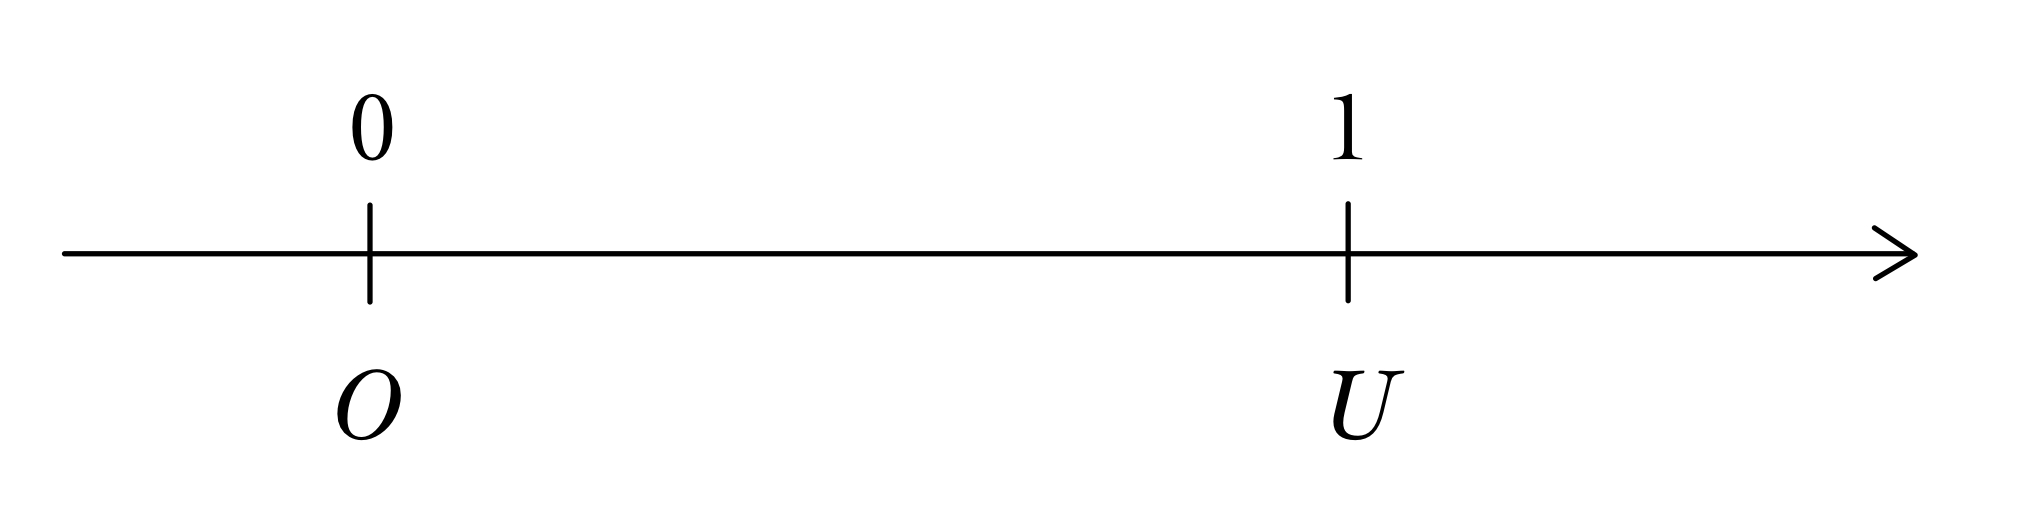
\includegraphics[width=0.5\textwidth]{number_line.PNG}\figtag{1.1.1}
\end{center}

In this manner we establish a one-to-one correspondence between the points of a line and the numbers of the real number system. Figure 1.2.2 shows some real numbers represented as points on the number line. Positive numbers appear to the right of $0$, negative numbers to the left of $0$.

\begin{center}
    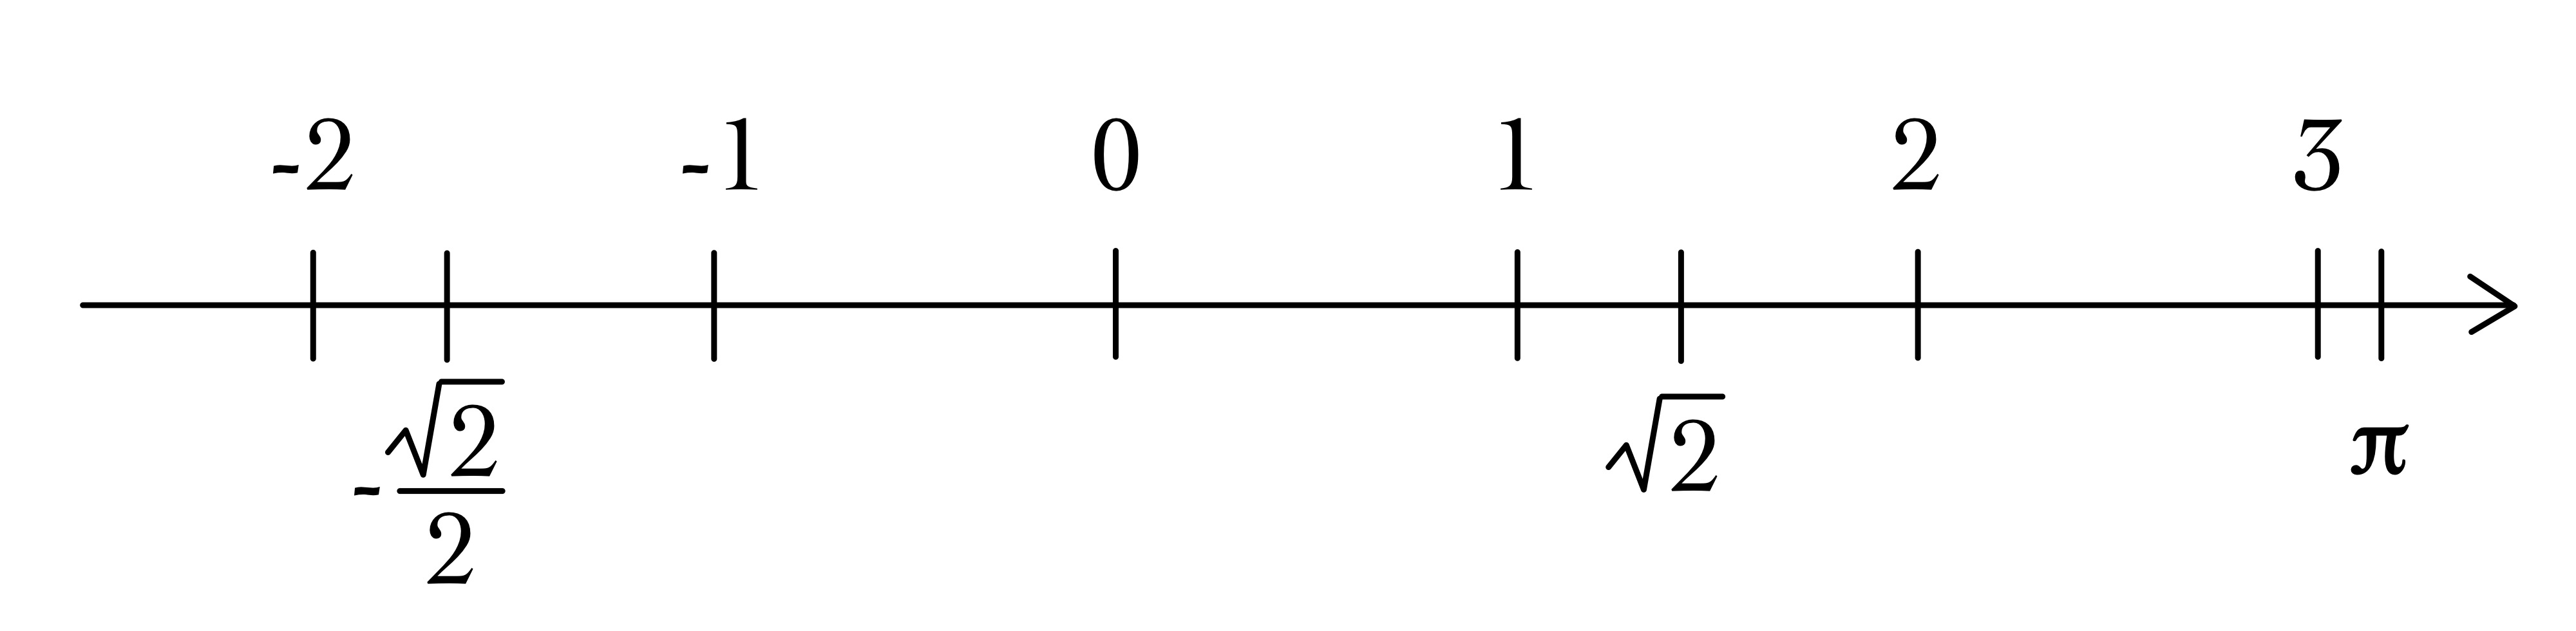
\includegraphics[width=0.65\textwidth]{number_line_example.JPG}\figtag{1.1.2}
\end{center}

\begin{exercise}
    Determine true or false for each of the following statements:
    \begin{enumerate}
        \item $1$ is the smallest positive integer.
        \item $-1$ is the smallest negative integer.
        \item $0$ is an integer.
        \item $1$ is the smallest positive integer.
    \end{enumerate}
\end{exercise}

\subsubsection*{Absolute Value}

Let $a\in\bbR$. The symbol $|a|$ is called ``the absolute value of $a$,'' and is defined by \vspace*{0.5em} \begin{equation*}
    |a|=\left\{\begin{array}{rl}a,&\quad\text{if $a\geq0$,}\\-a&\quad\text{if $a<0$.}\end{array}\right.\\[0.5em]
\end{equation*} The geometric meaning of $|a|$ is the distance between $a$ and $0$. Moreover, $|a-b|$ is the distance between $a$ and $b$.

We have some properties regarding the absolute values. 

\begin{theorem}
    Let $a, b\in\bbR$. The following statements always hold.
    \begin{enumerate}
        \item $|a|=0$ if and only if $a=0$.
        \item $|-a|=|a|$.
        \item $|ab|=|a||b|$.
        \item (\textit{Triangle Inequality}) $|a+b|\leq|a|+|b|$.
        \item (\textit{Reverse Triangle Inequality}) $||a|-|b||\leq|a-b|$.
        \item $|a^2|=|a|^2=a^2$.
    \end{enumerate}
\end{theorem}

\begin{exercise}
    Answer the following questions.
    \begin{enumerate}
        \item How many points are there is with unit length $4$ to the origin?
        \item Does the equation $\sqrt{a^2}=a$ hold for all $a\in\bbR$?
        \item Suppose moving $6$ meters to the right of the origin can be denoted as $+2$. How can moving $15$ meters to the left of the origin be denoted?
        \item There are three points $A$, $B$, and $C$ on the number line, with coordinate $1$, $6$, and $8$, respectively. Suppose one set the origin to $B$ without changing the unit lengh. What is the coordinate of $A$? What is the coordinate of $C$?
        \item If $a-b=18$ and $|a|=|b|$, what are $a$ and $b$?
        \item If $a$ and $b$ are with different signs, i.e., $ab<0$, and $|a|=|b|$, what is the value of $a+b$?
        \item Suppose $a$ and $b$ are all negative. If $|a|>|b|$, what is the order between $a$ and $b$?
    \end{enumerate}
\end{exercise}

\begin{exercise}
    Answer the following questions.
    \begin{enumerate}
        \item If $3|a+2|+2|b-7|=0$, what are $a$ and $b$?
        \item If $|4-a|=1$, what is $a$?
        \item If $a>0$, what is $|a|$?
        \item If $a<0$, what is $|a|$?
        \item How many integers $a$ are there satisfying $4<|a|<7$?
        \item How many integers $c$ are there satisfying $|c|\leq 4$?
        \item If $|a-2|=2$, what is $a$?
        \item If $|c+2|=8$, what is $c$?
    \end{enumerate}
\end{exercise}

\subsubsection*{Interval}

Accurately, intervals are connected subsets in the real number system. We use a pair of parentheses with a comma $(\cdot, \cdot)$ to indicate open intervals and use a pair of brackets with a comma $[\cdot, \cdot]$ to indicate closed intervals.

Suppose $a<b$. The open interval $(a, b)$ is the set of all numbers between $a$ and $b$: $$(a, b)=\{x\in\bbR\mid a<x<b\}.$$
\begin{center}
    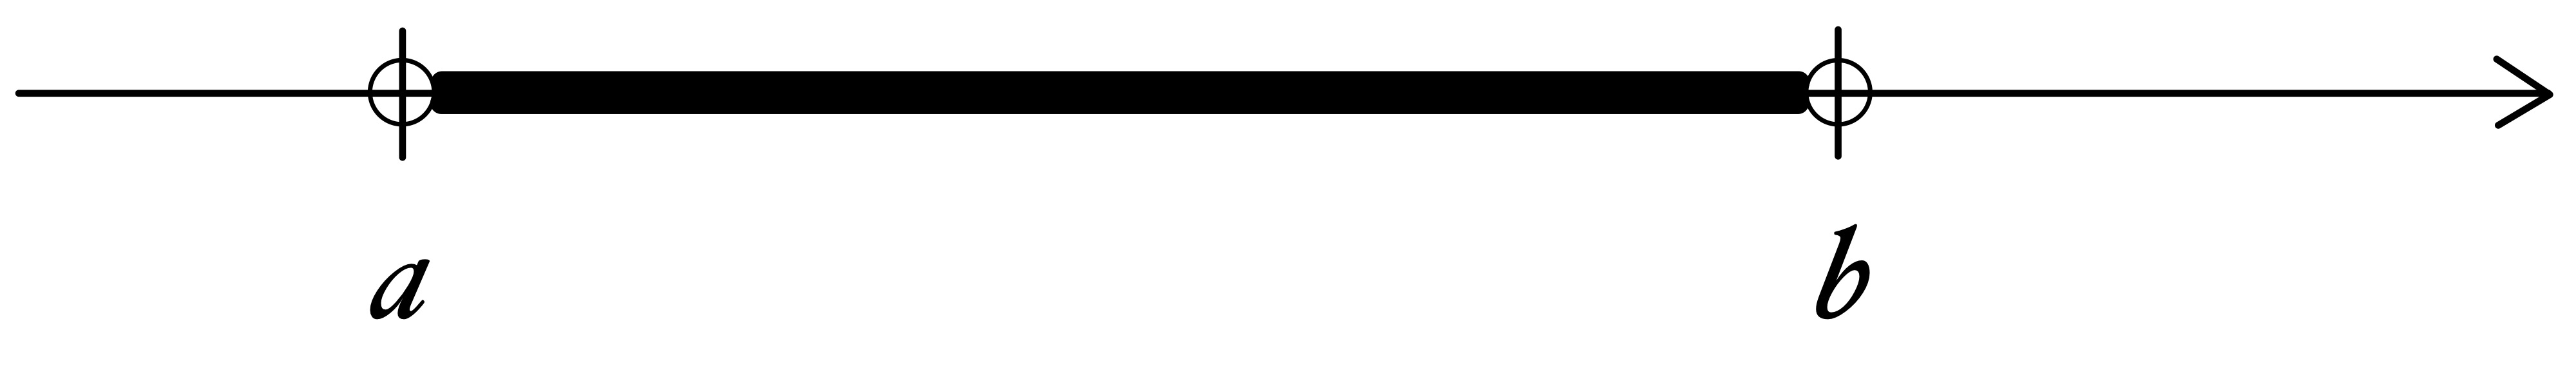
\includegraphics[width=0.45\textwidth]{interval_oo.JPG}
\end{center}
The closed interval $[a, b]$ is the open interval $(a, b)$ with endpoints $a$ and $b$: $$[a, b]=\{x\in\bbR\mid a\leq x\leq b\}.$$
\begin{center}
    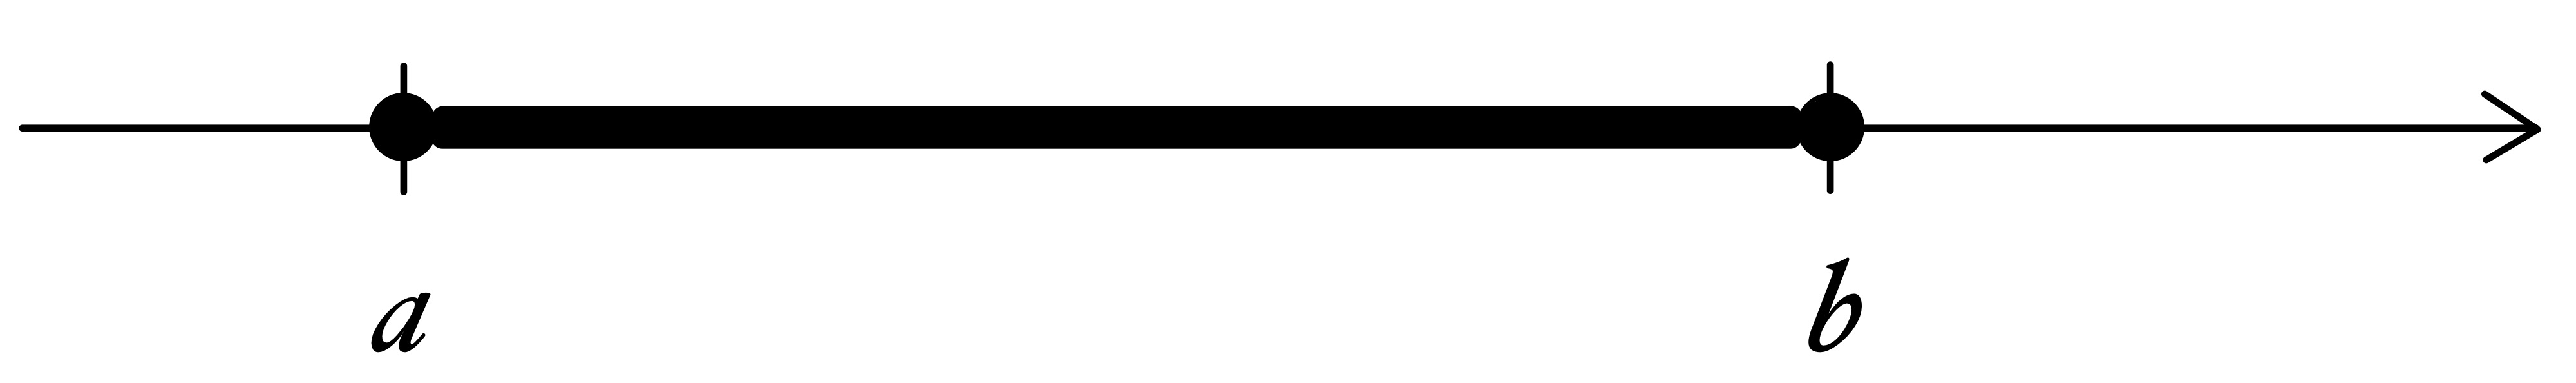
\includegraphics[width=0.45\textwidth]{interval_cc.JPG}
\end{center} We have seven more types of intervals: \begin{align*}
    (a, b]&=\{x\bbR\mid a<x\leq b\},\\
    [a, b)&=\{x\bbR\mid a\leq x<b\},\\
    (a, \infty)&=\{x\in\bbR\mid x>a\},\\
    [a, \infty)&=\{x\in\bbR\mid x\geq a\},\\
    (-\infty, b)&=\{x\in\bbR\mid x<b\},\\
    (-\infty, b]&=\{x\in\bbR\mid x\leq b\},\\
    (-\infty, \infty)&=\bbR.
\end{align*}

Interval notation is easy to remember: we use a square bracket to include an endpoint and a parenthesis to exclude it. On a number line, inclusion is indicated by a solid dot, exclusion by an open dot. The symbols $\infty$ and $-\infty$, read “infinity” and “negative infinity” (or “minus infinity”), do not represent real numbers. In the intervals listed above, the symbol $\infty$ is used to indicate that the interval extends indefinitely in the positive direction; the symbol $-\infty$ is used to indicate that the interval extends indefinitely in the negative direction.

\begin{exercise}
    Answer the following questions.
    \begin{enumerate}
        \item What is $[0, 2]\cap(2, 4)$?
        \item What is $[0, 1]\setminus(0, \infty)$?
        \item What is the set $A$ such that only elements $x$ in $A$ suffice $|x|\leq 3$?
    \end{enumerate}
\end{exercise}

\subsubsection*{Basic Algebra}

We use a small number on the top-right of another number to indicate the ``power'', which essentially means the number of multiplication.
\begin{notation}
    Let $r\in\bbR$ and $p\in\bbN$. The number $r^p$ is read ``$r$ to the power $p$'' and is with value $\overbrace{r\times r\times \cdots\times r}^{\text{$p$ times}}$. This explanation only works when the power is a positive integer.
\end{notation}

\begin{example}
    By the texts above, we have 
    \begin{enumerate}
        \item $(-2)^2=4$,
        \item $5^4=625$,
        \item $(-1)^5=-1$.
    \end{enumerate}
\end{example}

\begin{notation}
    Let $a>0$ and $p>0$. The number $a^{1/p}$ is called the $p$-th root of $a$ and is the number $b$ such that $b^q=a$; it can also be written as $\sqrt[q]{a}$. If $p=2$, we just write $\sqrt{a}$. The number $a^{-p}$ is the reciprocal of $a^p$.
\end{notation}

\begin{theorem}[Laws of Exponents]
    Let $a>0$ and $p, q\in\mathbb R$. The following always hold.
    \begin{enumerate}
        \item $a^{p+q}=a^p+a^q$.
        \item $a^{p-q}=\dfrac{a^p}{a^q}$.
        \item $(a^p)^q=a^{pq}$.
    \end{enumerate}
\end{theorem}

\begin{theorem}[Factorization]
    Let $a, b\in\bbR$. The following always hold.
    \begin{enumerate}
        \item $(a+b)^2=a^2+2ab+b^2$.
        \item $(a-b)^2=a^2-2ab+b^2$.
        \item $(a+b)^3=a^3+3a^2b+3ab^2+b^3$.
        \item $(a-b)^3=a^3-3a^2b+3ab^2-b^3$.
        \item $a^2-b^2=(a-b)(a+b)$.
        \item $a^3-b^3=(a-b)(a^2+ab+b^2)$.
        \item $a^n-b^n=(a-b)(a^{n-1}+a^{n-2}b+\cdots+ab^{n-2}+b^{n-1})$.
    \end{enumerate}
\end{theorem}


% Continuous limit
\chapter{Limits and Continuity}



% Formulae for derivatives
\chapter{Derivative and Differentiation}



% Graph drawing, l'Hospital
\chapter{Application of Differentiation}



% Formulae for antiderivatives
\chapter{Integral and Integration}



% sub, IBP
\chapter{Techniques of Integration}



\chapter{Numerical Sequences, Numerical Series, and Power Series}



\chapter{Multivariable Differentiation}



\chapter{Multiple Integrals}


\end{document}